\chapter{Networking}
The two key aspects of a network are:
\begin{enumerate}
   \item \textbf{Bandwidth} $\longrightarrow$ amount of data per second that can be moved through a specific connection
   \item \textbf{Latency} $\longrightarrow$ is the amount of time required for trasmitting data, measured from the moment it is sent from the source to the one it is available to the source.
\end{enumerate}
Latency ---in a datacenter--- to transmit data on the cable using \textit{``pure ethernet''} is of the order of $0.5\times10^{-6}s (\mu s)$.\\
If the TCP/IP stack is used (standard application case), latency is about $70-90\mu s$.

Furthermore, current drives have reached speeds such that latency may act as bottleneck between them and the CPU.

Cable aggregation (e.g. aggregating 4 cables 10Gbit/s, providing 40Gbit/s total)can be performed only at a low ---physical--- level. Otherwise the TCP/IP stream will be associated to a single cable of the ones aggregated, resulting in less bandwidth.


\section{Layers}
Programmers usually do not care about anything under layer 3/4 traffic.
However, in datacenters it is fundamental to understand how layer 2 works.
\note{Also because in datacenters there are no routers doing the work for you; you are building the fabric in the first place.}

Layer 2 is fundamental for 2 reasons:
\begin{enumerate}
   \item East-west is Ethernet in the datacenter
   \item All the dozens of protocols used in swithces are really used, so they are important.
   \item MTU - Maximum Transmission Unit
\end{enumerate}

\subsection{Protocols inside switches}
\begin{itemize}
   \item LLDP Link Layer Discovery Protocol - Allows to reconstruct at least partially the functioning of the network.4
   \item DCBX Data Center Bridging Exchange - A meta-protocol so that two devices can agree on the configuration of a bunch of protocols, tipically related to storage/data 
   \note{e.g. ``I need 50\% percent of the bandwidth otherwise a can't work''.\\
   It represents part of some kind of QoS for Ethernet}.
   \item PFC Priority Flow Control
   \item ETS Enhanced Transmission Selection
   \item RSTP Rapid Spanning Tree Protocol - Uses BPDU packets to explore the graph of the network and compute the spanning tree of the network and detect the ---malicious--- cycles if any.
\end{itemize}

This just to recall that \ul{the switch is not a stupid thing}! It is complex, fascinating, and deserves love; it's crucial to understand its functioning, also because its protocols occupy bandwidth.

\section{Ethernet Topology}
Typically nowdays the network is a \textbf{graph}, where internal nodes are switches or routers, and the leaves are servers.

The phyisical medium is no more shared, but conceptually the data link layer behaves as if it was.

On a switch, the only way to emulate a \textbf{shared bus}, is to \textit{``\textbf{copy-paste}''} a frame onto multiple ports, losing the ``identity'' of frames. Packets in higher layers (IP?) have an ID, but frames don't, making it impossible to recognize whether a frame is a copy of another one or not.
This approach makes \textbf{loops} a problem, because they disrupt performance by generating a packet storm.\\
The solution would be to ensure that the topology resembles a \textbf{tree}, instead of a graph.
\ul{But}, at the same time, \ul{a \textbf{fully connected graph}} allows to have \ul{multiple routes for the same destination}, possibly \ul{enhancing performance}, reducing ``hops'' before reaching the destination.

\subsection{\texttt{RSTP}}
\begin{center}
   \textit{So\dots how can we leave the graph to be connected, but making it a tree from a logical point of view?}

   The answer is the \texttt{RSTP} protocol.
\end{center}

RSTP sends \textit{probes} to understand whether there are loops and where are PCs located.

\subsection{Spine Leaf architecture}
\begin{figure}[htbp]
   \centering
   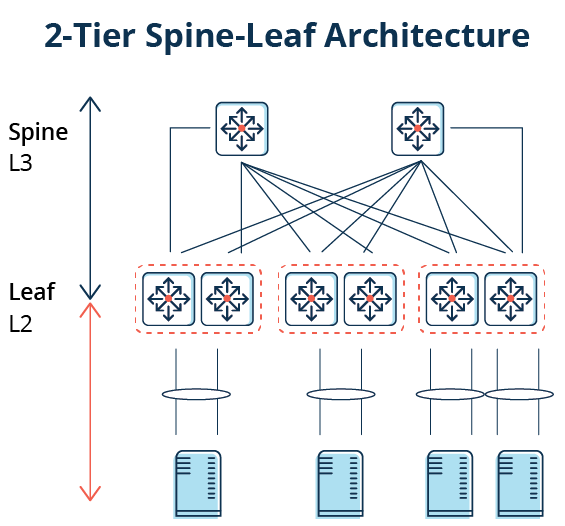
\includegraphics{images/spineleaf.png}
   \caption{Spine-leaf architecture schema (from \href{https://www.arubanetworks.com/faq/what-is-spine-leaf-architecture/}{Arubanetworks.com})}
   \label{fig:}
\end{figure}
A \textbf{spine-leaf} architecture is data center network topology that consists of two switching layers: a spine and leaf.
It ensures traffic is always the same number of hops from its next destination, so latency is lower and predictable (fixed).

Capacity also improves because STP is no longer required. While STP enables redundant paths between two switches, only one can be active at any time. As a result, paths often become oversubscribed. 
Conversely, spine-leaf architectures rely on protocols such as \textit{Equal-Cost Multipath} (\texttt{ECMP}) routing to load balance traffic across all available paths while still preventing network loops.

Spine-leaf allows \textit{scale-out} opposed to \textit{scale-up}, by adding additional spine switches, ultimately increasing capacity.

\subsection{Full fat tree}
In a ---full?--- \textbf{fat tree}, branches nearer the top of the hierarchy are "fatter" (thicker) than branches further down the hierarchy. In a telecommunications network, the branches are data links; the varied thickness (bandwidth) of the data links allows for more efficient and technology-specific use.

Full-fat tree is rarely needed.

\section{Virtualization}

With VLAN frames are extended by 4 bytes. Every switch nowdays automatically sets the \texttt{VLAN\_ID} to \texttt{1}; if the field is not existent, it is appended, making an \textbf{tagged} an \textit{untagged} frame.

Switches ensure that data cannot spill/leak from a VLAN to another.
VLAN became largely of use when 10Gbit connection came out, because only 1Gbit was a too constrained bandwidth to be splitted into multiple VLANs. 